\documentclass[tikz,convert={outfile=images/foldNatFree-mmorph-join.png,density=1000}]{standalone}
\usepackage[build={latexoptions={-output-directory=latex/png}}]{standalone}
\tikzset{
  ->/.style={draw=white!50!black,-stealth}
}
\tikzstyle{every node}=[color=white!50!black,font=\footnotesize]
\begin{document}
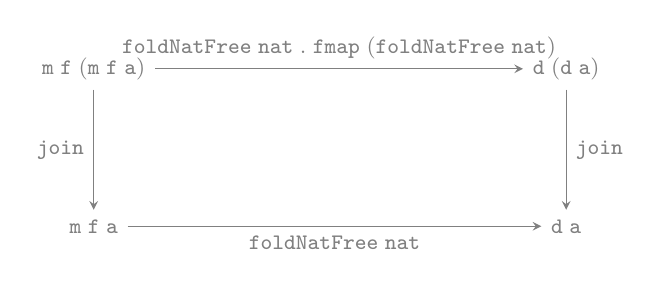
\begin{tikzpicture}
    \node (A) at (0,2) {\texttt{$\mathtt{m}\;\mathtt{f}\;(\mathtt{m}\;\mathtt{f}\;\mathtt{a})$}};
    \node (B) at (6,2) {\texttt{$\mathtt{d}\;(\mathtt{d}\;\mathtt{a})$}};
    \node (C) at (0,0) {\texttt{$\mathtt{m}\;\mathtt{f}\;\mathtt{a}$}};
    \node (D) at (6,0) {\texttt{$\mathtt{d}\;\mathtt{a}$}};
    \draw[->] (A) -- node[above]
    {$\mathtt{foldNatFree}\;\mathtt{nat}\;.\;\mathtt{fmap}\;(\mathtt{foldNatFree}\;\mathtt{nat})$} (B);
    \draw[->] (B) -- node[right] {$\mathtt{join}$} (D);
    \draw[->] (A) -- node[left] {$\mathtt{join}$} (C);
    \draw[->] (C) -- node[below] {$\mathtt{foldNatFree}\;\mathtt{nat}$} (D);
\end{tikzpicture}
\end{document}

